\documentclass[10pt,
t,
aspectratio=169]{beamer}

%%%%%%%%%%%%%%%%%%%%%%%%%%%%%%%%%% mode options %%%%%%%%%%%%%%%%%%%%%%%%%%%%%%%%

\mode<presentation>{\usetheme{uniS}}

% define a few pictures used throughout the slides
\pgfdeclareimage[width=0.7\paperwidth]{background}{images/jason-rosewell-ASKeuOZqhYU-unsplash.jpg}  % background picture for title slide
\pgfdeclareimage[height=1cm]{unilogo}{unilogo.pdf} % UniS logo for title slide
\pgfdeclareimage[height=1cm]{unilogow}{unilogo_w.pdf} % (white) UniS logo for final slide
\pgfdeclareimage[width=2.5cm]{speaker}{images/Clifton_Headshot.jpg} % speaker photo for final slide

%%%%%%%%%%%%%%%%%%%%%%%%%%%%%%%%%% misc stuff %%%%%%%%%%%%%%%%%%%%%%%%%%%%%%%%%%

% automatically display \sectionpage at beginning of every \section{}
\AtBeginSection[]{%
\begin{frame}[plain]
  \sectionpage
\end{frame}
}

% set up an image credit
\newcommand{\simplecaption}[1]{\parbox{\textwidth}{\scriptsize\color{darkgray} #1}}
\newcommand{\givecredit}[1]{\parbox{\textwidth}{\tiny\color{gray} #1}}
% underline links
\usepackage{ulem}
\renewcommand{\ULdepth}{1.8pt}
\newcommand{\textlink}[2]{\href{#1}{\uline{#2}}}
% ORCID logo
\newcommand{\orcid}[1]{\href{https://orcid.org/#1}{
\includegraphics[height=10pt]{images/ORCIDiD_icon128x128.png}}}
% LinkedIn logo
\newcommand{\linkedin}[1]{\href{#1}{
\includegraphics[height=10pt]{images/LI-In-Bug.png}}}
% enable overlapping images
% see https://tex.stackexchange.com/questions/34921/how-to-overlap-images-in-a-beamer-slide
\def\Put(#1,#2)#3{\leavevmode\makebox(0,0){\put(#1,#2){#3}}}

%---------------------------------------------------------------
% Packages
%---------------------------------------------------------------
\usepackage{booktabs}
\usepackage{fontspec}
\usepackage{fontawesome}
\usepackage{transparent}

%%%%%%%%%%%%%%%%%%%%%%%%%%%%%%%%%%%% setup %%%%%%%%%%%%%%%%%%%%%%%%%%%%%%%%%%%%%

\title[Communications strategies]{
    LIKE\\
    Open Science Course\\
    Seminar 4:\\
    Communications Strategies}
\author[Andy Clifton]{Dr.-Sc.\\ Andrew Clifton}
\institute{Institute of Aircraft Design (IFB), University of Stuttgart}
\date{10 November 2020}

%---------------------------------------------------------------
% DOCUMENT STARTS HERE
%---------------------------------------------------------------

\begin{document}

\begin{frame}[plain]
  \titlepage
\end{frame}


% Table of contents
\begin{frame}
  \frametitle{Today's discussion}
    \tableofcontents
    \vfill
    \givecredit{Cover page photo by \textlink{ https://unsplash.com/@jasonrosewell}{Jason Rosewell} on \textlink{https://unsplash.com/s/photos/communications}{Unsplash}}
\end{frame}

% content
\section[The course]{The LIKE Open Science Course}
\stepcounter{subsection} %We don't use subsection titles, only frametitles
\label{sec:course}

%---------------------------------------------------------------
% 1. What is open science?
%---------------------------------------------------------------
\begin{frame}{What is this ``Open Science'' thing anyway?}

\begin{quotation}<1->
Open science is the movement to make scientific research and its dissemination accessible to all levels of an inquiring society, amateur or professional. \\
Open science is transparent and accessible knowledge that is shared and developed through collaborative networks.
\begin{flushright}
    \tiny{---\textlink{https://en.wikipedia.org/wiki/Open_science}{Wikipedia}}
  \end{flushright}
\end{quotation}

\begin{columns}
    \begin{column}{.45\textwidth}
    % it is...
        \begin{block}<2->{It is...}
            \begin{itemize}
                \item A philosophy
                \item A set of tools
                \item An old idea
            \end{itemize}
        \end{block}
    \end{column}
    
    \begin{column}{.45\textwidth}
    % it is not...
        \begin{block}<2->{It is not...}
            \begin{itemize}
                \item Difficult
                \item Expensive
                \item Rewarded directly
            \end{itemize}
        \end{block}
    \end{column}
    
\end{columns}

\end{frame}


%---------------------------------------------------------------
% 2. High-level goals
%---------------------------------------------------------------

% high-level goals
\begin{frame}{Course goals}

\begin{columns}[t]
    % LHS text
    \begin{column}{.45\textwidth}

    \textbf{We want you to be successful.}
    \vspace{3ex}
    

    This course will:
    \begin{itemize}
        \item Tell you about open science
        \item Give you a toolbox
        \item Help you use these tools
    \end{itemize}
    
    \end{column}

    % RHS image
    \begin{column}{.45\textwidth}

        \centering
        
\includegraphics[width=0.8\textwidth]{images/milan-popovic-BmyXTxyDL-I-unsplash.jpg}
    
        \givecredit{\centering Photo by \textlink{https://unsplash.com/@itsmiki5?utm_source=unsplash&amp;utm_medium=referral&amp;utm_content=creditCopyText}{Milan Popovic} on \textlink{https://unsplash.com/s/photos/tools?utm_source=unsplash&amp;utm_medium=referral&amp;utm_content=creditCopyText}{Unsplash}}
    
    \end{column}

\end{columns}


\end{frame}

%---------------------------------------------------------------
% 3. Calendar
%---------------------------------------------------------------

\begin{frame}{Course outline}

\begingroup
\renewcommand{\arraystretch}{0.9} % Default value: 1
\setlength\tabcolsep{0pt}  % default value: 6pt
% Table based on https://github.com/LIKE-ITN/OpenScienceTrainingCourse/blob/master/readme.md#course-outline
\setlength{\fboxsep}{3pt}
\colorbox{uniSgray!10}{%

    \begin{tabular}{@{}p{0.35\textwidth}p{0.35\textwidth}p{0.3\textwidth}@{}}
        Seminar & Self-study & Deliverable \\
        \midrule
        1. \textlink{https://github.com/LIKE-ITN/OpenScienceTrainingCourse/blob/master/01_seminar1/readme.md}{Introducing open science} &  &  \\
         &  1. \textlink{https://github.com/LIKE-ITN/OpenScienceTrainingCourse/blob/master/selfstudy1.md}{Background reading} &  \\
        2. \textlink{https://github.com/LIKE-ITN/OpenScienceTrainingCourse/blob/master/seminar2.md}{Guiding principles} &  &  \\
         & 2. \textlink{https://github.com/LIKE-ITN/OpenScienceTrainingCourse/blob/master/selfstudy2.md}{Is your group's work FAIR?} &  \\
        3. \textlink{https://github.com/LIKE-ITN/OpenScienceTrainingCourse/blob/master/seminar3.md}{Open science and intellectual property} &  &  \\
         & 3. \textlink{https://github.com/LIKE-ITN/OpenScienceTrainingCourse/blob/master/selfstudy3.md}{Implementing open science} & \\
        4. \textlink{https://github.com/LIKE-ITN/OpenScienceTrainingCourse/blob/master/seminar3.md}{Communicating your science} &  &  \\
         & 4. \textlink{https://github.com/LIKE-ITN/OpenScienceTrainingCourse/blob/master/selfstudy4.md}{Communications strategies} &  \\
         &  & 1. \textlink{https://github.com/LIKE-ITN/OpenScienceTrainingCourse/blob/master/deliverable1.md}{Implementation case study} \\
         5. \textlink{https://github.com/LIKE-ITN/OpenScienceTrainingCourse/blob/master/seminar5.md}{What are data management plans and why do they matter?} &  &   \\
         & 5. \textlink{https://github.com/LIKE-ITN/OpenScienceTrainingCourse/blob/master/selfstudy5.md}{Draft a data management plan} &  \\
        Workshop: \textlink{https://github.com/LIKE-ITN/OpenScienceTrainingCourse/blob/master/workshop1.md}{Open science in LIKE} &  & \\
         & 6. \textlink{https://github.com/LIKE-ITN/OpenScienceTrainingCourse/blob/master/selfstudy6.md}{Revise data management plan} &  \\
         &  & 2. \textlink{https://github.com/LIKE-ITN/OpenScienceTrainingCourse/blob/master/deliverable2.md}{Data management plan} \\
         
    \end{tabular}
}\endgroup

\end{frame}

%---------------------------------------------------------------
% 3. Logistics - Office Hours, Questions, Etc.
%---------------------------------------------------------------

\begin{frame}{Course logistics}
    
    \begin{columns}
    \column{.45\textwidth}
   
        \begin{block}{Grading}
            \begin{itemize}
                \item No exams, but..
                \item Deliverables needed for a participation certificate.
            \end{itemize}
        \end{block}

        \begin{block}{Questions?}
            \begin{itemize}
                \item No office hours!
                \item Use slack and ask each other
            \end{itemize}
        \end{block}

    \column{.45\textwidth}
    
        \begin{block}{Errors, suggestions, corrections...}
            \begin{itemize}
                \item  \textlink{https://github.com/LIKE-ITN/OpenScienceTrainingCourse/issues}{Help improve the material}
            \end{itemize}
        \end{block}

        \begin{block}{Your feedback}
        This is a new course!
            \begin{itemize}
                \item Get in touch at any time
                \item Survey at the end
            \end{itemize}
        \end{block}

        \end{columns}
    
\end{frame}

\section{Introduction}
\label{sec:introduction}

%---------------------------------------------------------------
% 0. Motivating statement
%---------------------------------------------------------------
\begin{frame}[plain,c]
\begin{center}
    \Huge{If no-one knows you did it,\\%
    you didn't do it.}
\end{center}
\end{frame}

%---------------------------------------------------------------
% 1. Seminar outline
%---------------------------------------------------------------
\begin{frame}{Our goals for today}
    
    \begin{columns}[c]
        \begin{column}{.45\textwidth}
        
        Learn how to promote your work by crafting and executing a communications strategy
        
            \begin{itemize}
                \item Why do we communicate?
                \item How do we communicate?
                \item What do we communicate?
            \end{itemize}
        \end{column}
        
        \begin{column}{.45\textwidth}
            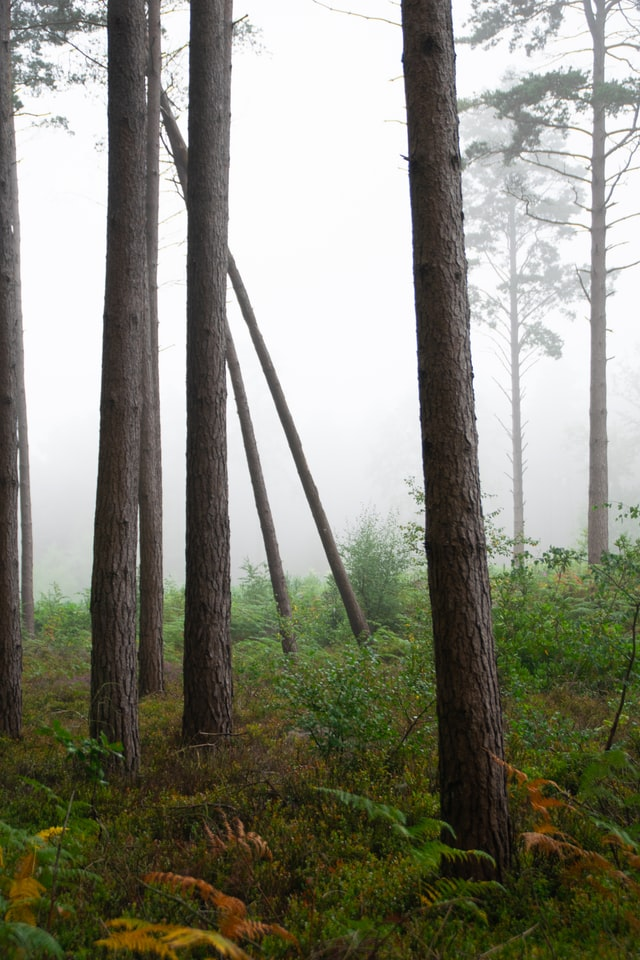
\includegraphics[trim=0cm 1cm 2.5cm 5cm, clip=true,width=0.85\textwidth]{images/harry-shelton-PmwG9GmNyaU-unsplash.jpg}
            
            \givecredit{Photo by \textlink{https://unsplash.com/@itsharryshelton}{Harry Shelton} on \textlink{https://unsplash.com}{Unsplash}}
        \end{column}
    \end{columns}
    
\end{frame}

%---------------------------------------------------------------
% 2. People
%---------------------------------------------------------------

\begin{frame}{Who's here?}
    
    \begin{columns}[t]
        \begin{column}{.3\textwidth}
    
            \begin{block}{Andy Clifton}
            \centering
            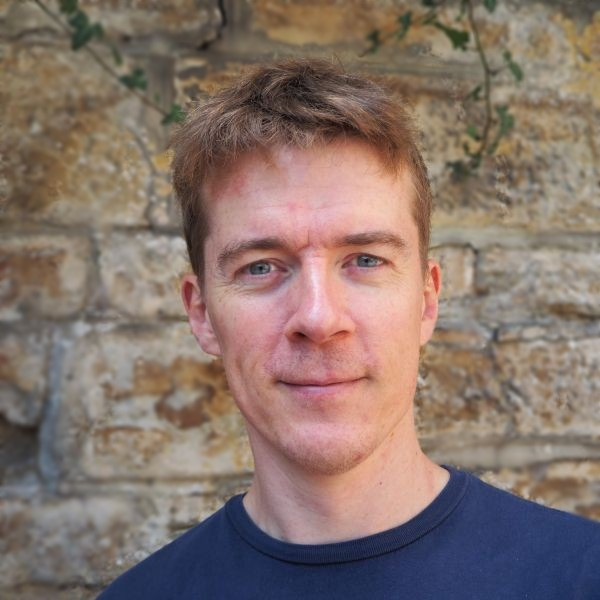
\includegraphics[width=0.8\textwidth]{images/Clifton_Headshot.jpg}\\
            IEA Wind Task 32\\ Operating Agent \\
            \orcid{0000-0001-9698-5083}
            \linkedin{http://www.linkedin.com/in/andyclifton}
            \end{block}
        \end{column}
   
        \begin{column}{.3\textwidth}
            \begin{block}{Nikola Vasiljevic}
            \centering
            
\includegraphics[width=0.8\textwidth]{images/Vasiljevic_Headshot.png}\\
            Special Consultant for Digitalization \\
            \orcid{0000-0002-9381-9693}
            \linkedin{https://dk.linkedin.com/in/niva83}
            \end{block}
        \end{column}
        
        \begin{column}{.3\textwidth}
            \begin{block}{And you}
            \centering
            {\fontsize{100}{120}\selectfont\faUsers}\\
            Please introduce yourselves!
            \end{block}
        \end{column}
    \end{columns}

\end{frame}
\section[Communications strategies]{Telling people about your work}
\stepcounter{subsection} %We don't use subsection titles, only frametitles
\label{sec:communications_strategies}

%---------------------------------------------------------------
% 1. Why do we communicate
%---------------------------------------------------------------

\begin{frame}{Why do we communicate?}

% left empty for student input

\end{frame}

%---------------------------------------------------------------
% 2. Effective communications 
%---------------------------------------------------------------
\begin{frame}{Effective communications make a difference}

\vspace{-0.75cm}
\begin{columns}

    \begin{column}{0.3\textwidth}
        \begin{block}{They make you aware}
        \centering
            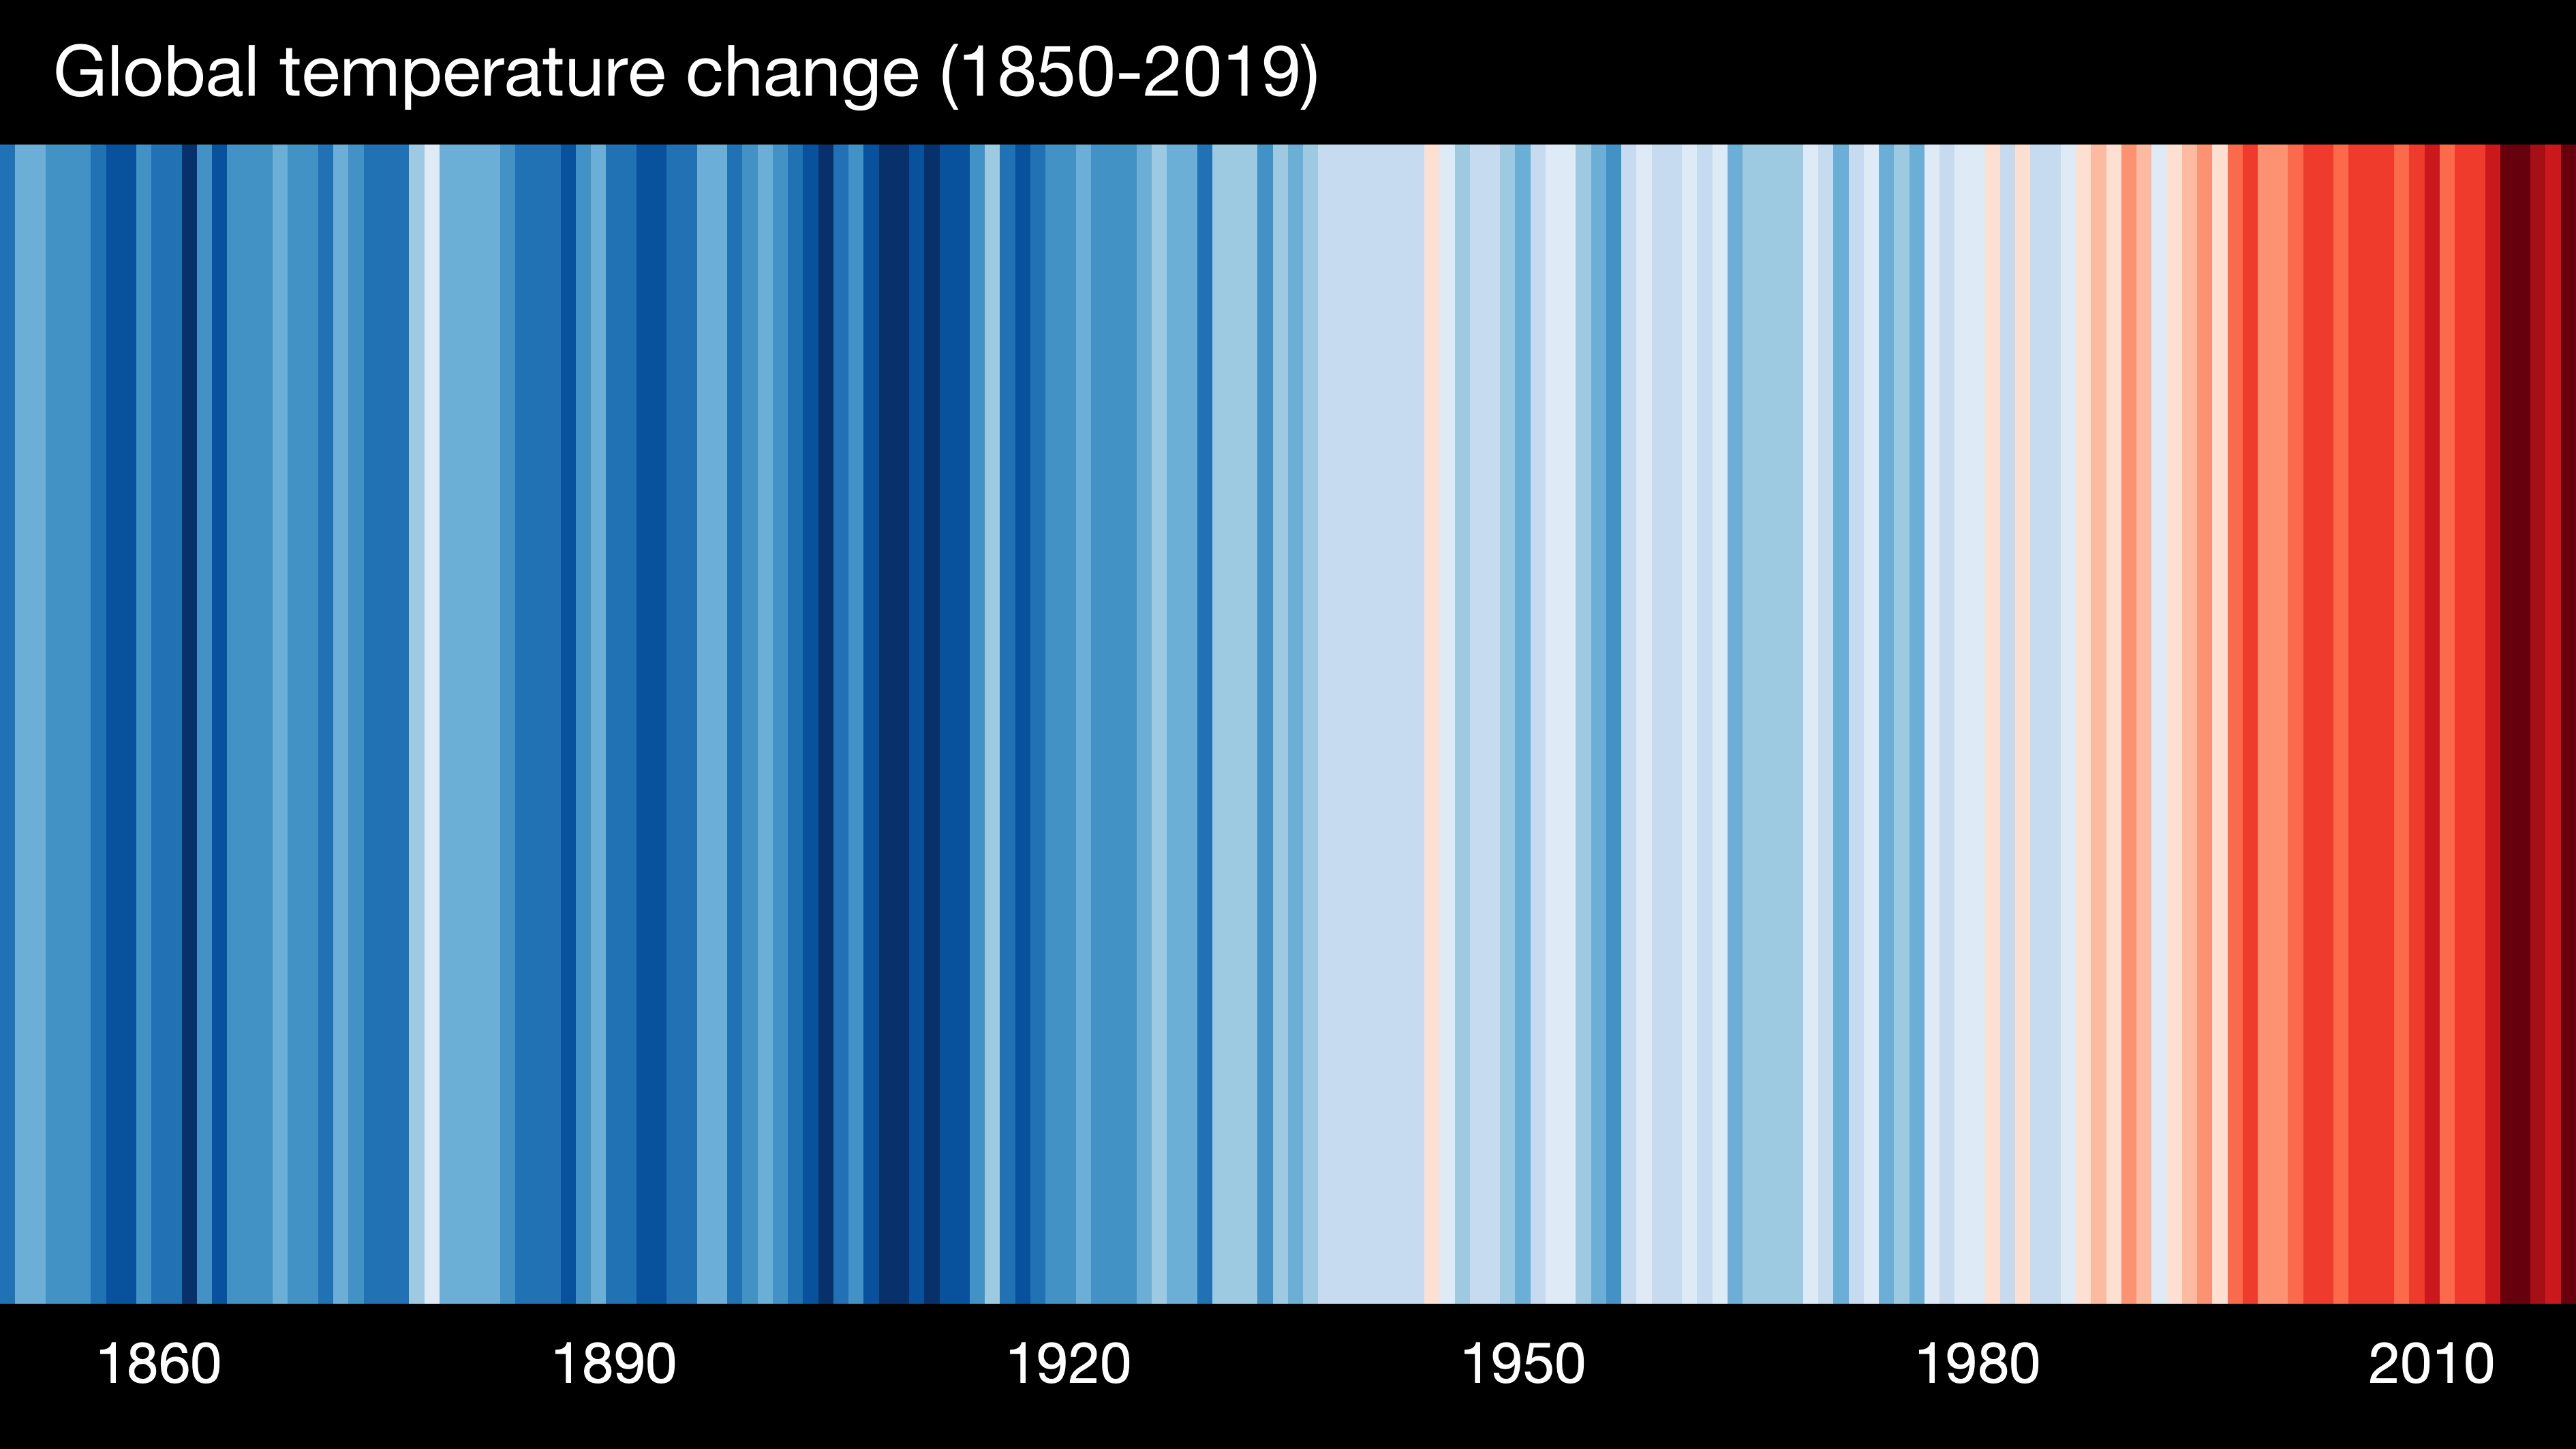
\includegraphics[width=\textwidth]{images/_stripes_GLOBE---1850-2019-MO-withlabels.png}
            \givecredit{\textlink{https://showyourstripes.info/}{Annual average temperatures for the globe}. Image by Ed Hawkins (University of Reading). Used under CC BY 4.0 license.}
        \end{block}
    \end{column}
    
    \begin{column}{0.3\textwidth}
        \begin{block}{They make you care}
        \centering
            
\includegraphics[width=\textwidth]{images/mika-baumeister-9fJidQI2o-s-unsplash.jpg}
            \givecredit{Photo by \textlink{https://unsplash.com/@mbaumi}{Mika Baumeister} on \textlink{https://unsplash.com}{Unsplash}}
        \end{block}
    \end{column}

    \begin{column}{0.3\textwidth}
        \begin{block}{They make you act}
        \centering
            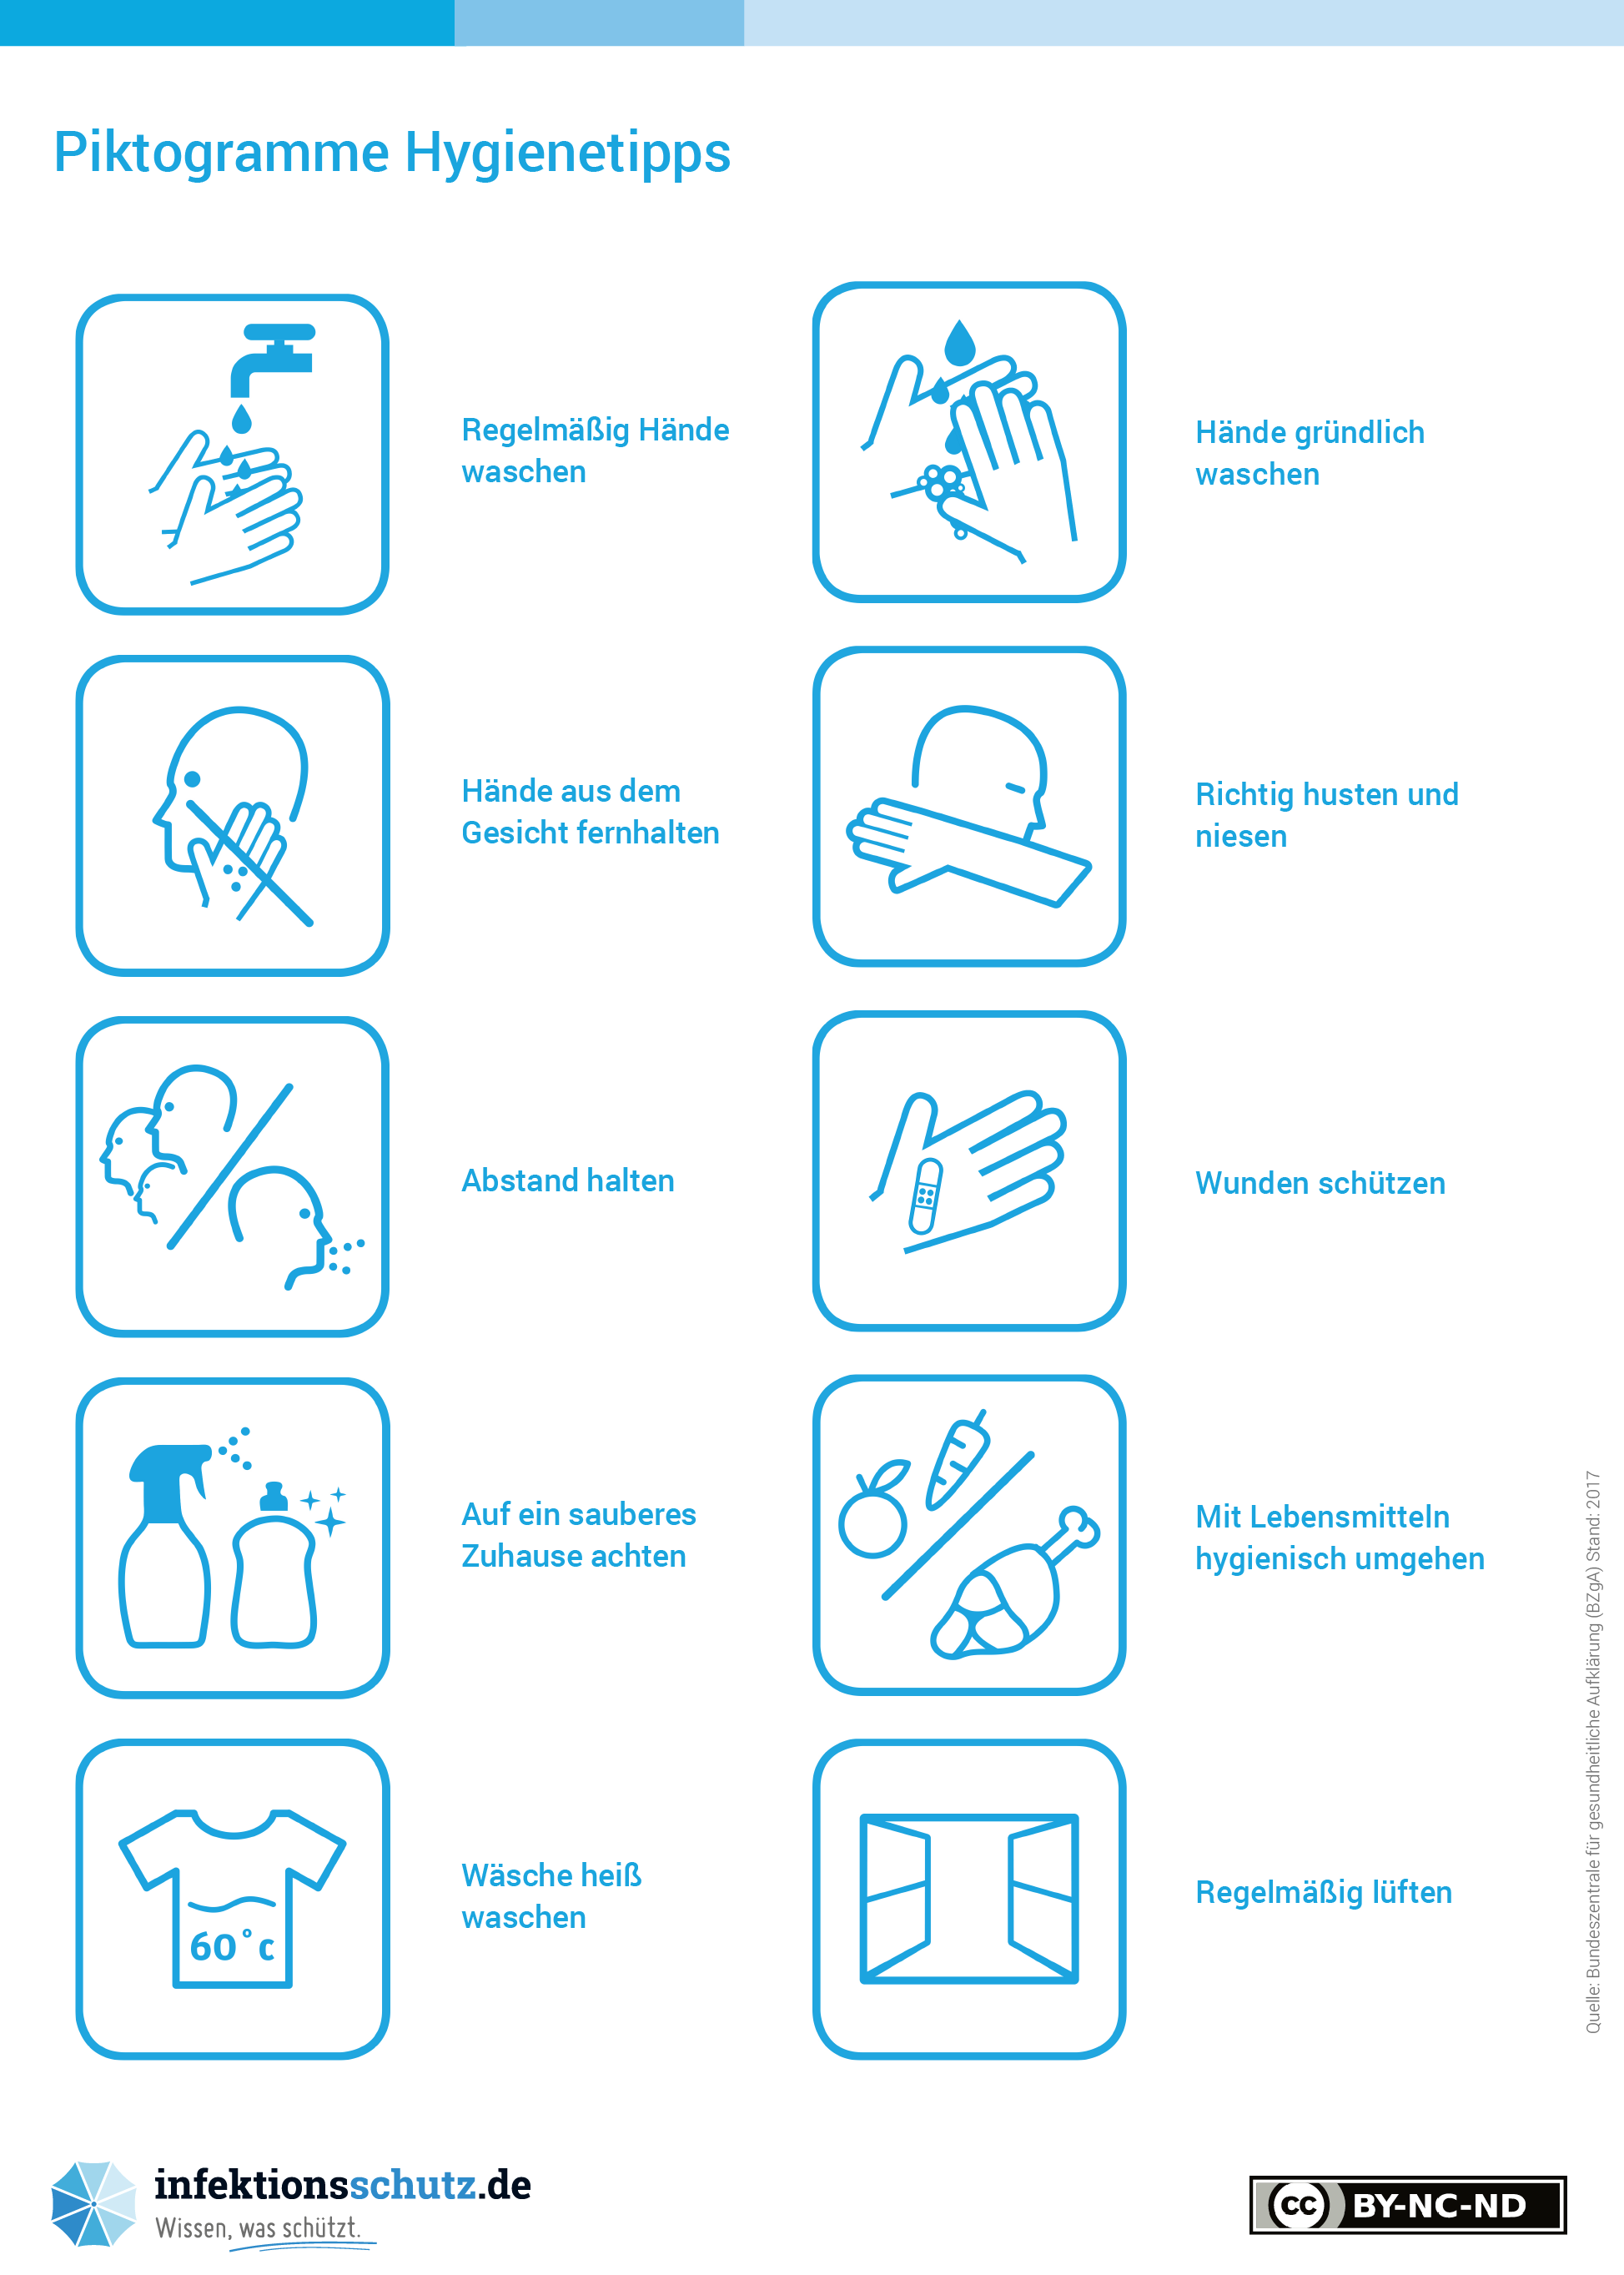
\includegraphics[width=\textwidth]{images/Piktogramme_Hygienetipps_300dpi.png}
            \givecredit{\textlink{https://www.infektionsschutz.de/mediathek/infografiken.html}{German Federal Centre for Health Education (BZgA)}}
        \end{block}

    \end{column}

\end{columns}

\end{frame}

%---------------------------------------------------------------
% 3. How we make effective communications
%---------------------------------------------------------------
\begin{frame}{Getting started}

\begin{columns}

    \begin{column}{0.45\textwidth}
        \begin{minipage}[t][.7\textheight]{\textwidth}
        
        Figure out why you are communicating:
        \begin{itemize}
            \item Who's the audience?
            \item What do you want them to do?
            \item How does your communication help?
        \end{itemize}
        \vfill
        Work out how to achieve that goal:
        \begin{itemize}
            \item Inform
            \item Persuade
            \item Provoke
        \end{itemize}
        \vfill
        Choose your media
        \vfill
        Tell your story
        \end{minipage}
    \end{column}

    \begin{column}{0.45\textwidth}

    \end{column}

\end{columns}


\end{frame}

%---------------------------------------------------------------
% 4. Communications campaigns
%---------------------------------------------------------------
\begin{frame}[plain]
% blog post + linkedin + article + uni press release

\centering
% image illustrating a communications campaign

\usetikzlibrary{positioning}
\usetikzlibrary{overlay-beamer-styles}

\begin{tikzpicture}[remember picture, overlay]

    % NREL press release
    \node[anchor=south west, xshift=0.25cm](NREL) at (current page.south west) {
        
\includegraphics[height=150pt]{images/eaau2027_NREL_pressrelease.png}
    };

    % DTU press release
    \node[anchor=north west](DTU) at (current page.north west) {
        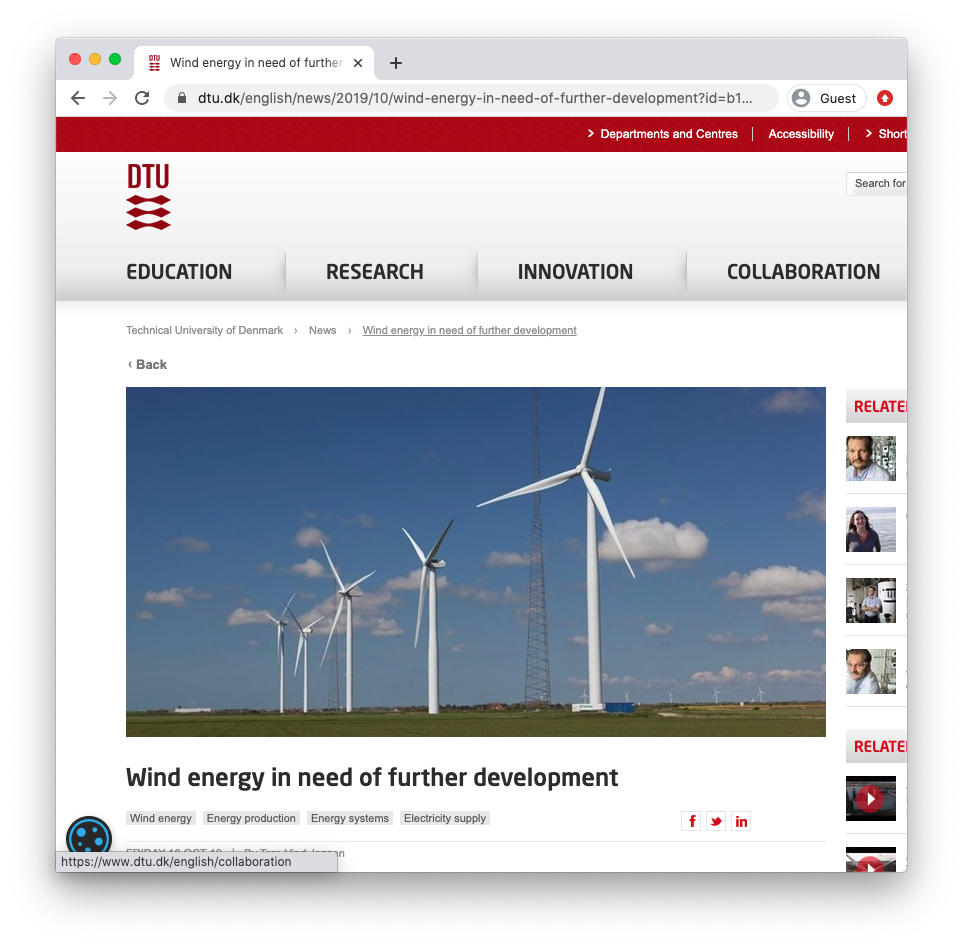
\includegraphics[height=150pt]{images/eaau2027_DTU_pressrelease.png}
    };
    
    % Conference picture
    \node[anchor=north east, xshift=-0.25cm](Conf) at (current page.east) {
        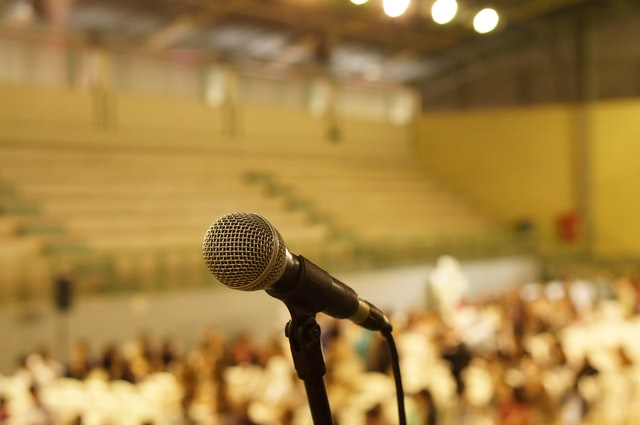
\includegraphics[height=100pt]{images/joao-cruz-IkEpl3JkVqU-unsplash.jpg}
    };
    
    % Article from wind power monthly
    \node[anchor=north east](WPM) at (current page.north east) {
        
\includegraphics[height=150pt]{images/eaau2027_WPM.png}
    };
    
    % linkedin logo
    \node[anchor=east, yshift=-0.75cm](L) at (current page.east) {
        \colorbox{white}{
\includegraphics[height=25pt]{images/LI-Logo.png}}
    };
    
    
    % paper
    \node[line width=1mm](Sci) at (current page.center) {
        \frame{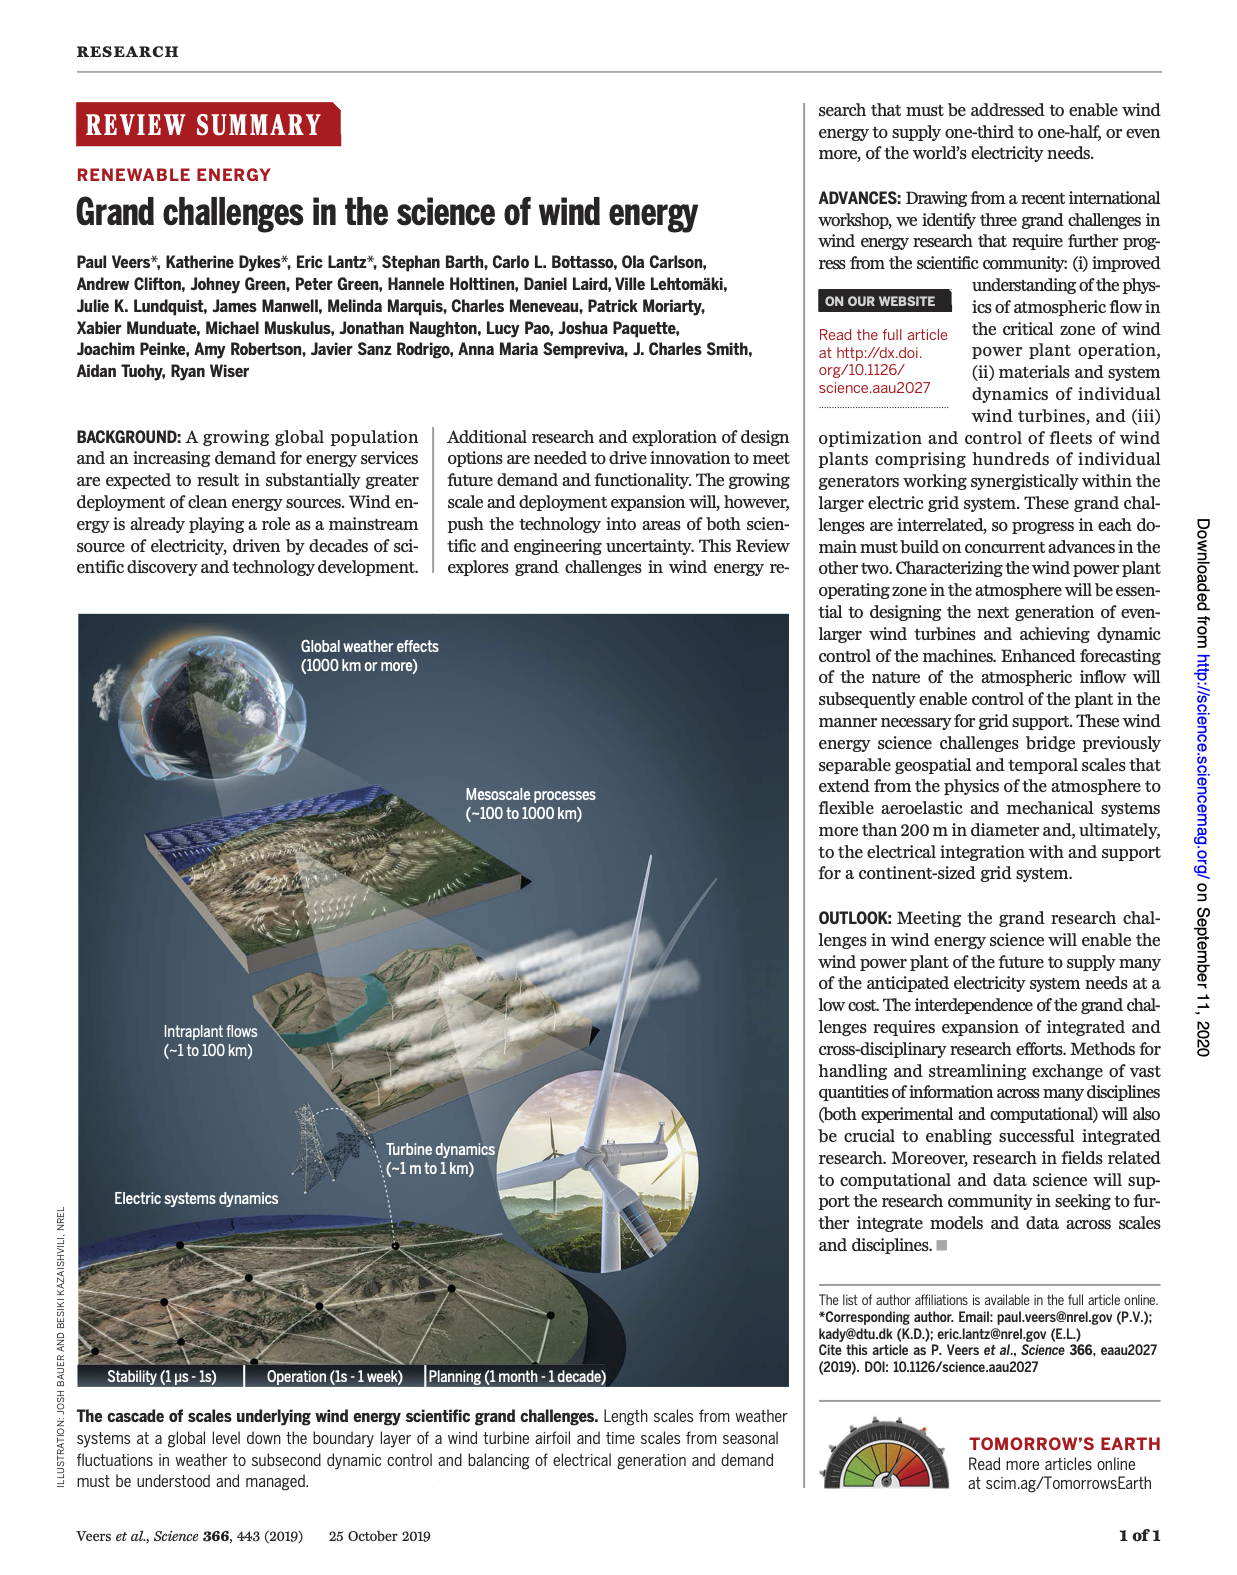
\includegraphics[height=0.9\paperheight]{images/eaau2027_front.png}}
    };    

\end{tikzpicture}


\end{frame}

%---------------------------------------------------------------
% 5. Media
%---------------------------------------------------------------

\begin{frame}{Channel - Audience - Message}

\vspace{-0.75cm}
\begin{columns}
    \begin{column}{0.3\textwidth}
        \begin{block}{Apps \& mobile devices}
            \centering
            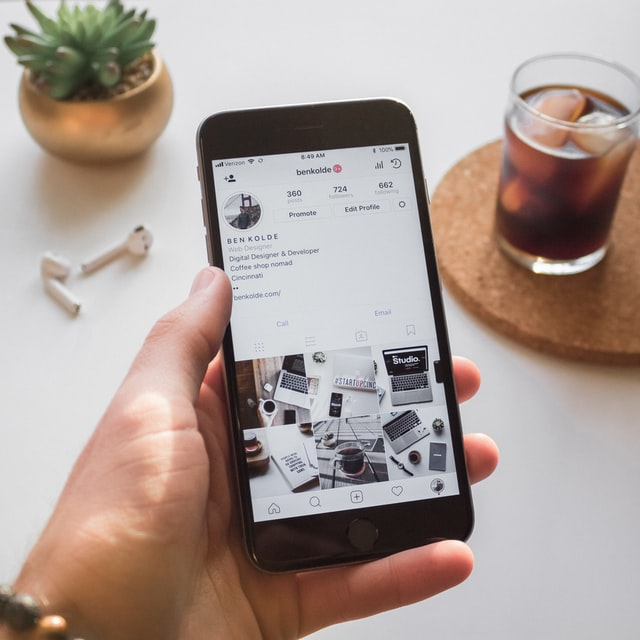
\includegraphics[width=\textwidth]{images/ben-kolde-_zqJaEyo6I4-unsplash.jpg}
            \givecredit{Photo by \textlink{https://unsplash.com/@benkolde}{Ben Kolde} on \textlink{https://unsplash.com}{Unsplash}}
            % some text about the message
            {\small
            \textbf{Audience:} Almost anyone\\
            \textbf{Message:} Call to action. %
            }
        \end{block}
    \end{column}
    
    \begin{column}{0.3\textwidth}
        \begin{block}{Conferences \& Webinars}
        \centering
            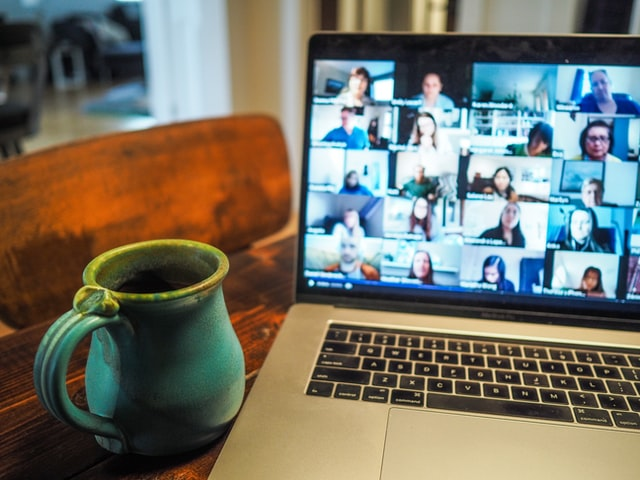
\includegraphics[width=\textwidth]{images/chris-montgomery-smgTvepind4-unsplash.jpg}
            \givecredit{Photo by \textlink{https://unsplash.com/@cwmonty}{Chris Montgomery} on \textlink{https://unsplash.com}{Unsplash}}
            % some text about the message
            {\small
            \textbf{Audience:} Already interested\\
            \textbf{Message:} Insight \& understanding. %
            }
        \end{block}
    \end{column}
    
    \begin{column}{0.3\textwidth}
        \begin{block}{Print*}
        \centering
            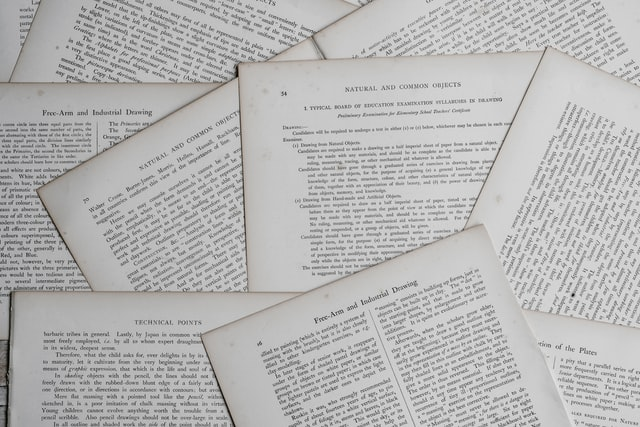
\includegraphics[width=\textwidth]{images/annie-spratt-5cFwQ-WMcJU-unsplash.jpg}
            \givecredit{Photo by \textlink{https://unsplash.com/@anniespratt}{Annie Spratt} on \textlink{https://unsplash.com}{Unsplash}}
            % some text about the message
            {\small
            \textbf{Audience:} \emph{Really} interested\\
            \textbf{Message:} Actionable information. %
            }
        \end{block}
    \end{column}
    
\end{columns}

\end{frame}

%---------------------------------------------------------------
% 6. New Media
%---------------------------------------------------------------

\begin{frame}{Are there better ways to reach your audience?}
\centering
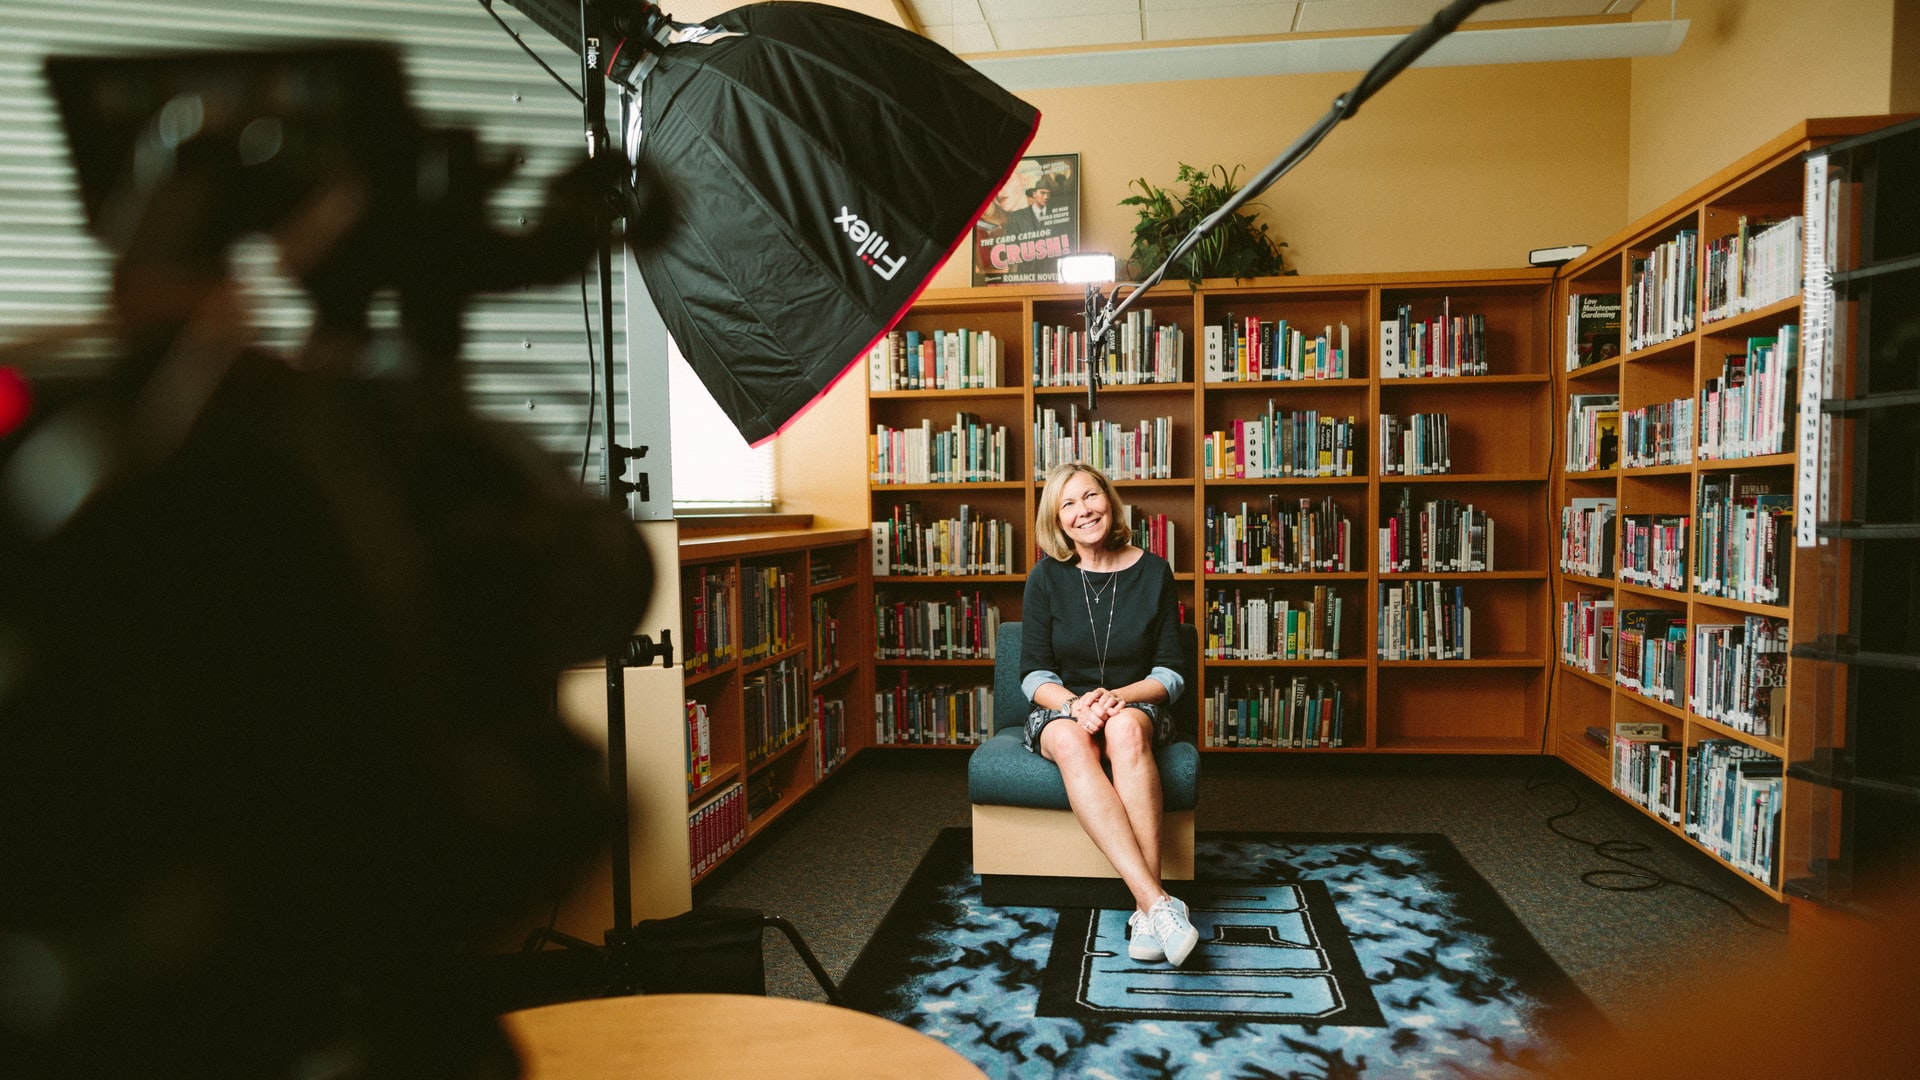
\includegraphics[height=0.7\textheight]{images/sam-mcghee-4siwRamtFAk-unsplash.jpg}

\givecredit{Photo by \textlink{https://unsplash.com/@sammcghee}{Sam McGhee} on \textlink{https://unsplash.com}{Unsplash}}
\end{frame}


\section[Closing]{Closing thoughts}
\label{sec:closing}

%---------------------------------------------------------------
% 1. Summary
%---------------------------------------------------------------
\begin{frame}{Seminar summary}

	\begin{columns}[c]
		% lessons
		\begin{column}{.45\textwidth}
		    You've learned:
		    \begin{itemize}
			    \item About the course
			    \item A first definition for ``open science''
			    \item How openness helps fight COVID-19
			    \item Some challenges with being open
		    \end{itemize}
		\end{column}

		\begin{column}{.45\textwidth}
		
		    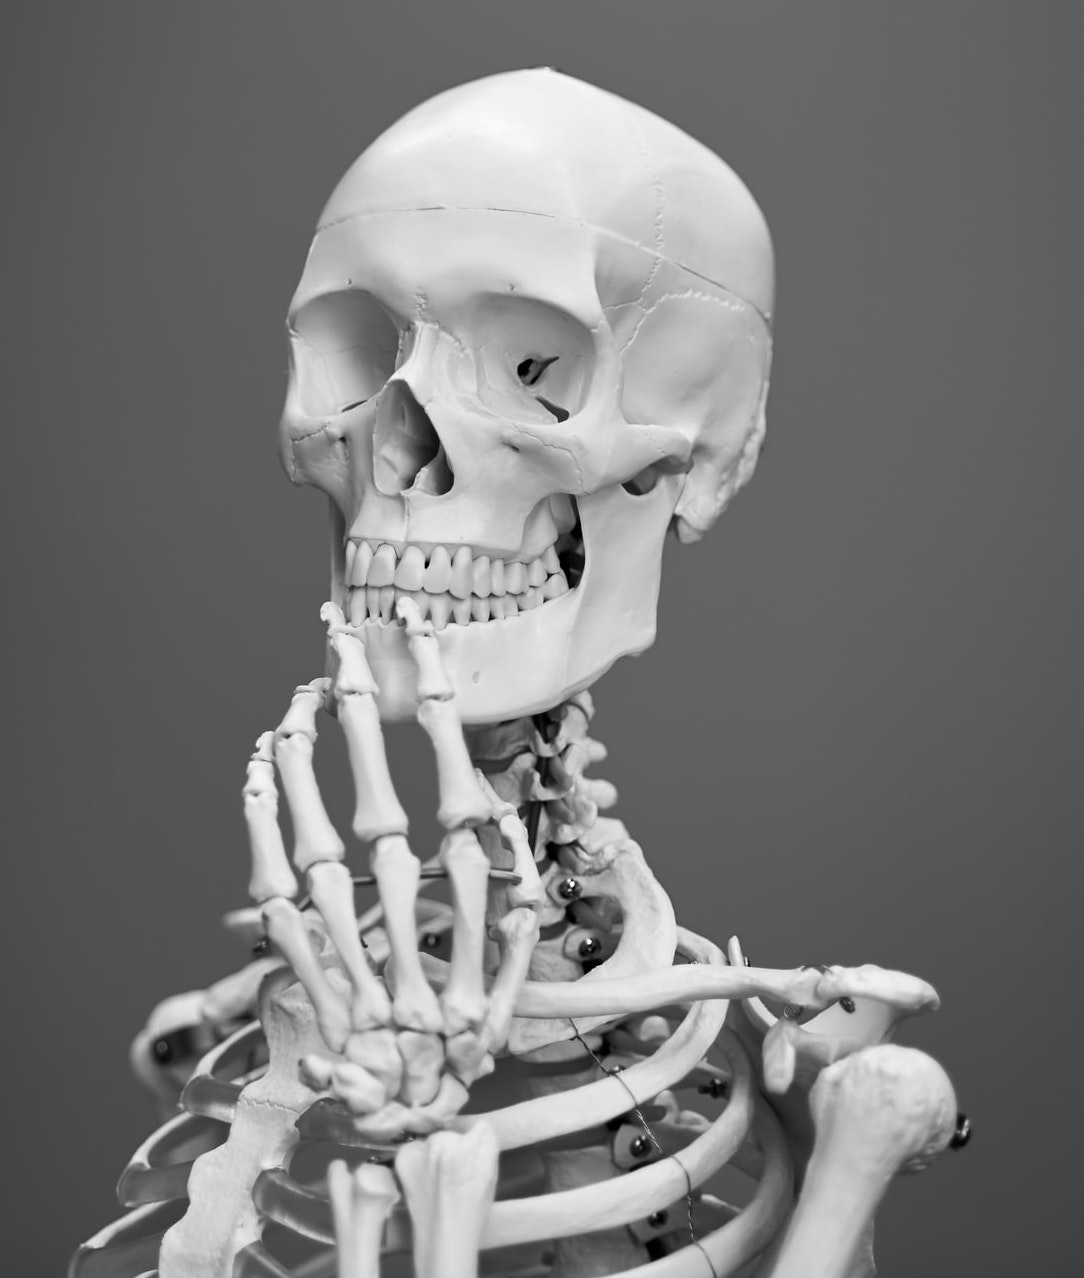
\includegraphics[width=0.85\textwidth]{images/mathew-schwartz-8rj4sz9YLCI-unsplash-crop.jpg}
		    
		    \givecredit{%
		        \centering
		        Photo by \textlink{https://unsplash.com/@cadop}{Mathew Schwartz} on \textlink{https://unsplash.com/s/photos/thinking}{Unsplash}}
		\end{column}
		
	\end{columns}

\end{frame}

%---------------------------------------------------------------
% 2. Next steps
%---------------------------------------------------------------

\begin{frame}{What to do now}

	\begin{columns}[t]
		\column{.45\textwidth}
		\begin{block}{Self study 1: Background reading}
			Read about how open science has been used to fight COVID-19, for example...
			\begin{itemize}
				\item \textlink{https://www.nature.com/articles/d41586-020-01246-3}{Open science takes on the coronavirus pandemic (Nature, 2020)}
				\item \textlink{https://www.rd-alliance.org/data-sharing-time-pandemic-patterns-preview-rda-covid-19-group-results}{``Data Sharing in a Time of Pandemic''} (Patterns, 2020)
				\item \textlink{https://home.cern/news/news/computing/open-science-against-covid-19-how-zenodo-and-openaire-support-scientists}{``Open Science against COVID-19: how Zenodo and OpenAIRE support the scientists''} (CERN, 2020)
			\end{itemize}
		\end{block}

		\column{.45\textwidth}
		\begin{block}{Seminar 2: Guiding principles}
			What are the basic principles of open science? How can you implement them, and what do they mean for your organisation?
			\begin{itemize}
				\item \textlink{https://github.com/LIKE-ITN/OpenScienceTrainingCourse/blob/master/seminar2.md}{Seminar materials on GitHub}
			\end{itemize}
		\end{block}

	\end{columns}

\end{frame}

%---------------------------------------------------------------
% 3. Let's make this open
%---------------------------------------------------------------
\begin{frame}{Let's make this presentation open}

	\begin{columns}[t]
		\begin{column}{.45\textwidth}
		    \centering
		    
\includegraphics[height=1.5cm]{images/1280px-FAIR_data_principles.jpg}

		    \givecredit{\centering Image source: \textlink{https://en.wikipedia.org/wiki/FAIR_data#/media/File:FAIR_data_principles.jpg}{Wikimedia}. Credit: \textlink{https://commons.wikimedia.org/w/index.php?title=User:SangyaPundi}{SangyaPundir}. \\
		    Reused under the \textlink{https://creativecommons.org/licenses/by-sa/4.0}{CC BY-SA 4.0 license}}
		\end{column}

		\begin{column}{.45\textwidth}
		    \centering
		    
\includegraphics[height=1.5cm]{images/cc-by-sa.png}
        \end{column}
	\end{columns}

	\begin{columns}[t]
		\begin{column}{.45\textwidth}
		    \centering
		% Findable
		    \begin{block}{Findable}
			    This presentation has a DOI:
		    \end{block}

		    % accessible
		    \begin{block}{Accessible}
			    This presentation is archived at Zenodo.org. \\
			    The source code is available through GitHub.
		    \end{block}
        \end{column}

		\begin{column}{.45\textwidth}
		    \centering
		    \begin{block}{Interoperable}
			    This material is produced using the \LaTeX\space `Beamer' package.
		    \end{block}

		    \begin{block}{Reusable}
			    This material is reusable under the \textlink{https://creativecommons.org/licenses/by/4.0/}{CC-BY-4.0 license}.
		    \end{block}
        \end{column}
	\end{columns}
\end{frame}

% corporate identity
\finalslide{clifton@ifb.uni-stuttgart.de}{+49 711 685 683 25}{www.uni-stuttgart.de/windenergie}

\end{document}




%%% Local Variables:
%%% mode: latex
%%% TeX-master: t
%%% End:
